\chapter*{Сейсморазведка}
\addcontentsline{toc}{chapter}{Сейсморазведка}



Сейсмическая разведка (сейсморазведка) - это геофизический метод исследования строения земной коры, поисков и разведки залежей нефти и газа, а также других полезных ископаемых. Для изучения внутреннего строения Земли необходимо использовать процессы, несущие информацию из ее глубинных слоев на поверхность. При этом наиболее подходящими являются процессы, которые в наибольшей степени локализованы в пространстве. Такими процессами прежде всего являются упругие волны, распространяющиеся через Землю, а длина волны определяет разрешающую способность метода.

Методика сейсморазведки основана на изучении кинематики волн или времени пробега различных волн от пункта их возбуждения до сейсмоприемников, улавливающих скорости смещения почвы, и их динамики или интенсивности волн. Основные два метода: метод отраженных волн (МОВ) и метод преломленных волн (МПВ). По решаемым задачам различают глубинную, структурную, нефтегазовую, рудную, инженерную сейсморазведки; по месту проведения сейсморазведка подразделяется на наземную (полевую), акваториальную (морскую), скважинную и подземную, а по частотам колебаний упругих волн можно выделить высокочастотную, среднечастотную и низкочастотную. Чем выше частота упругих волн, тем больше их затухание и меньше глубинность разведки.






Извлечение полезной информации из сейсмических записей происходит в процессе их обработки и интерпретации. От качества выполнения этой работы зависят полнота, надежность и точность получаемых геологических результатов.

Принципиальной основной обработки экспериментальных сейсморазведочных данных служит решение обратных задач. Обратная задача - это определение строения сейсмогеологической среды по наблюдениям возникающего в ней поля упругих волн.

Идеальным решением этой задачи явилось бы установление истинного распределения скоростных и поглощающих свойств горных пород о всем объеме изучаемой геологической среды. Однако на практике такой результат недостижим из-за ряда ограничений принципиального характера, среди которых наиболее существенны следующие: нехватка граничных условий, дискретность системы наблюдений, неидеальная математическая модель, предел разрешающей способности приборов, искажения информации, извлекаемой из экспериментальных данных.

Указанные обстоятельства ограничивают полноту и точность решения обратной задачи. Однако в рамках этих ограничений существуют реальные возможности получения по сейсмическим наблюдениям достаточно надежных количественных данных о строении сложных геологических объектов. Задача теории обработки сейсморазведочной информации - обеспечить наилучшую реализацию этих возможностей.



\section*{Основы изучения строения Земли}
\addcontentsline{toc}{section}{Основы изучения строения Земли}



В Земле могут распространяться механические (сейсмические) и электромагнитные волны, которые не позволяют зондировать недра Земли. Сейсмология дает наиболее полную и подробную информацию о строении Земли. Именно поэтому построение различных моделей Земли опирается на сейсмическую модель - скоростной разрез Земли.

Традиционно в сейсморазведке наибольшее применение нашли объемные волны (Рис. \ref{1-1}):
\begin{itemize}
	\item продольная: частицы колеблются в направлении распространение волны (волна сжатия - растяжения);
	\item поперечная: частицы колеблются в направлении, перпендикулярном распространению волны (волна сдвига).
\end{itemize}
Известны также поверхностные волны (Рис. \ref{1-2}), называемые волнами Рэлея (R) и Лява (L). Эти волны резко затухают с глубиной.

Формулы для скорости объемных волн:
\begin{equation}
	\begin{aligned}
	c_P = \sqrt{\dfrac{K + 4/3\mu}{\rho}}~&-~для~продольных~P-волн, \\
	c_S = \sqrt{\dfrac{\mu}{\rho}}~&-~для~поперечных~S-волн,
	\end{aligned}
\end{equation}
где $K$ - модуль всестороннего сжатия (объемный модуль); $\mu$ - модуль сдвига; $\rho$ - плотность.

Так как всегда $c_P > c_S$, то и прямые продольные волны также всегда приходят на регистрацию раньше прямых поперечных от того же источников, отсюда их названия: P (primary) - первичная и S (secondary) - вторичная.

\begin{figure}[H]
	\centering
	\begin{subfigure}{.6\textwidth}
		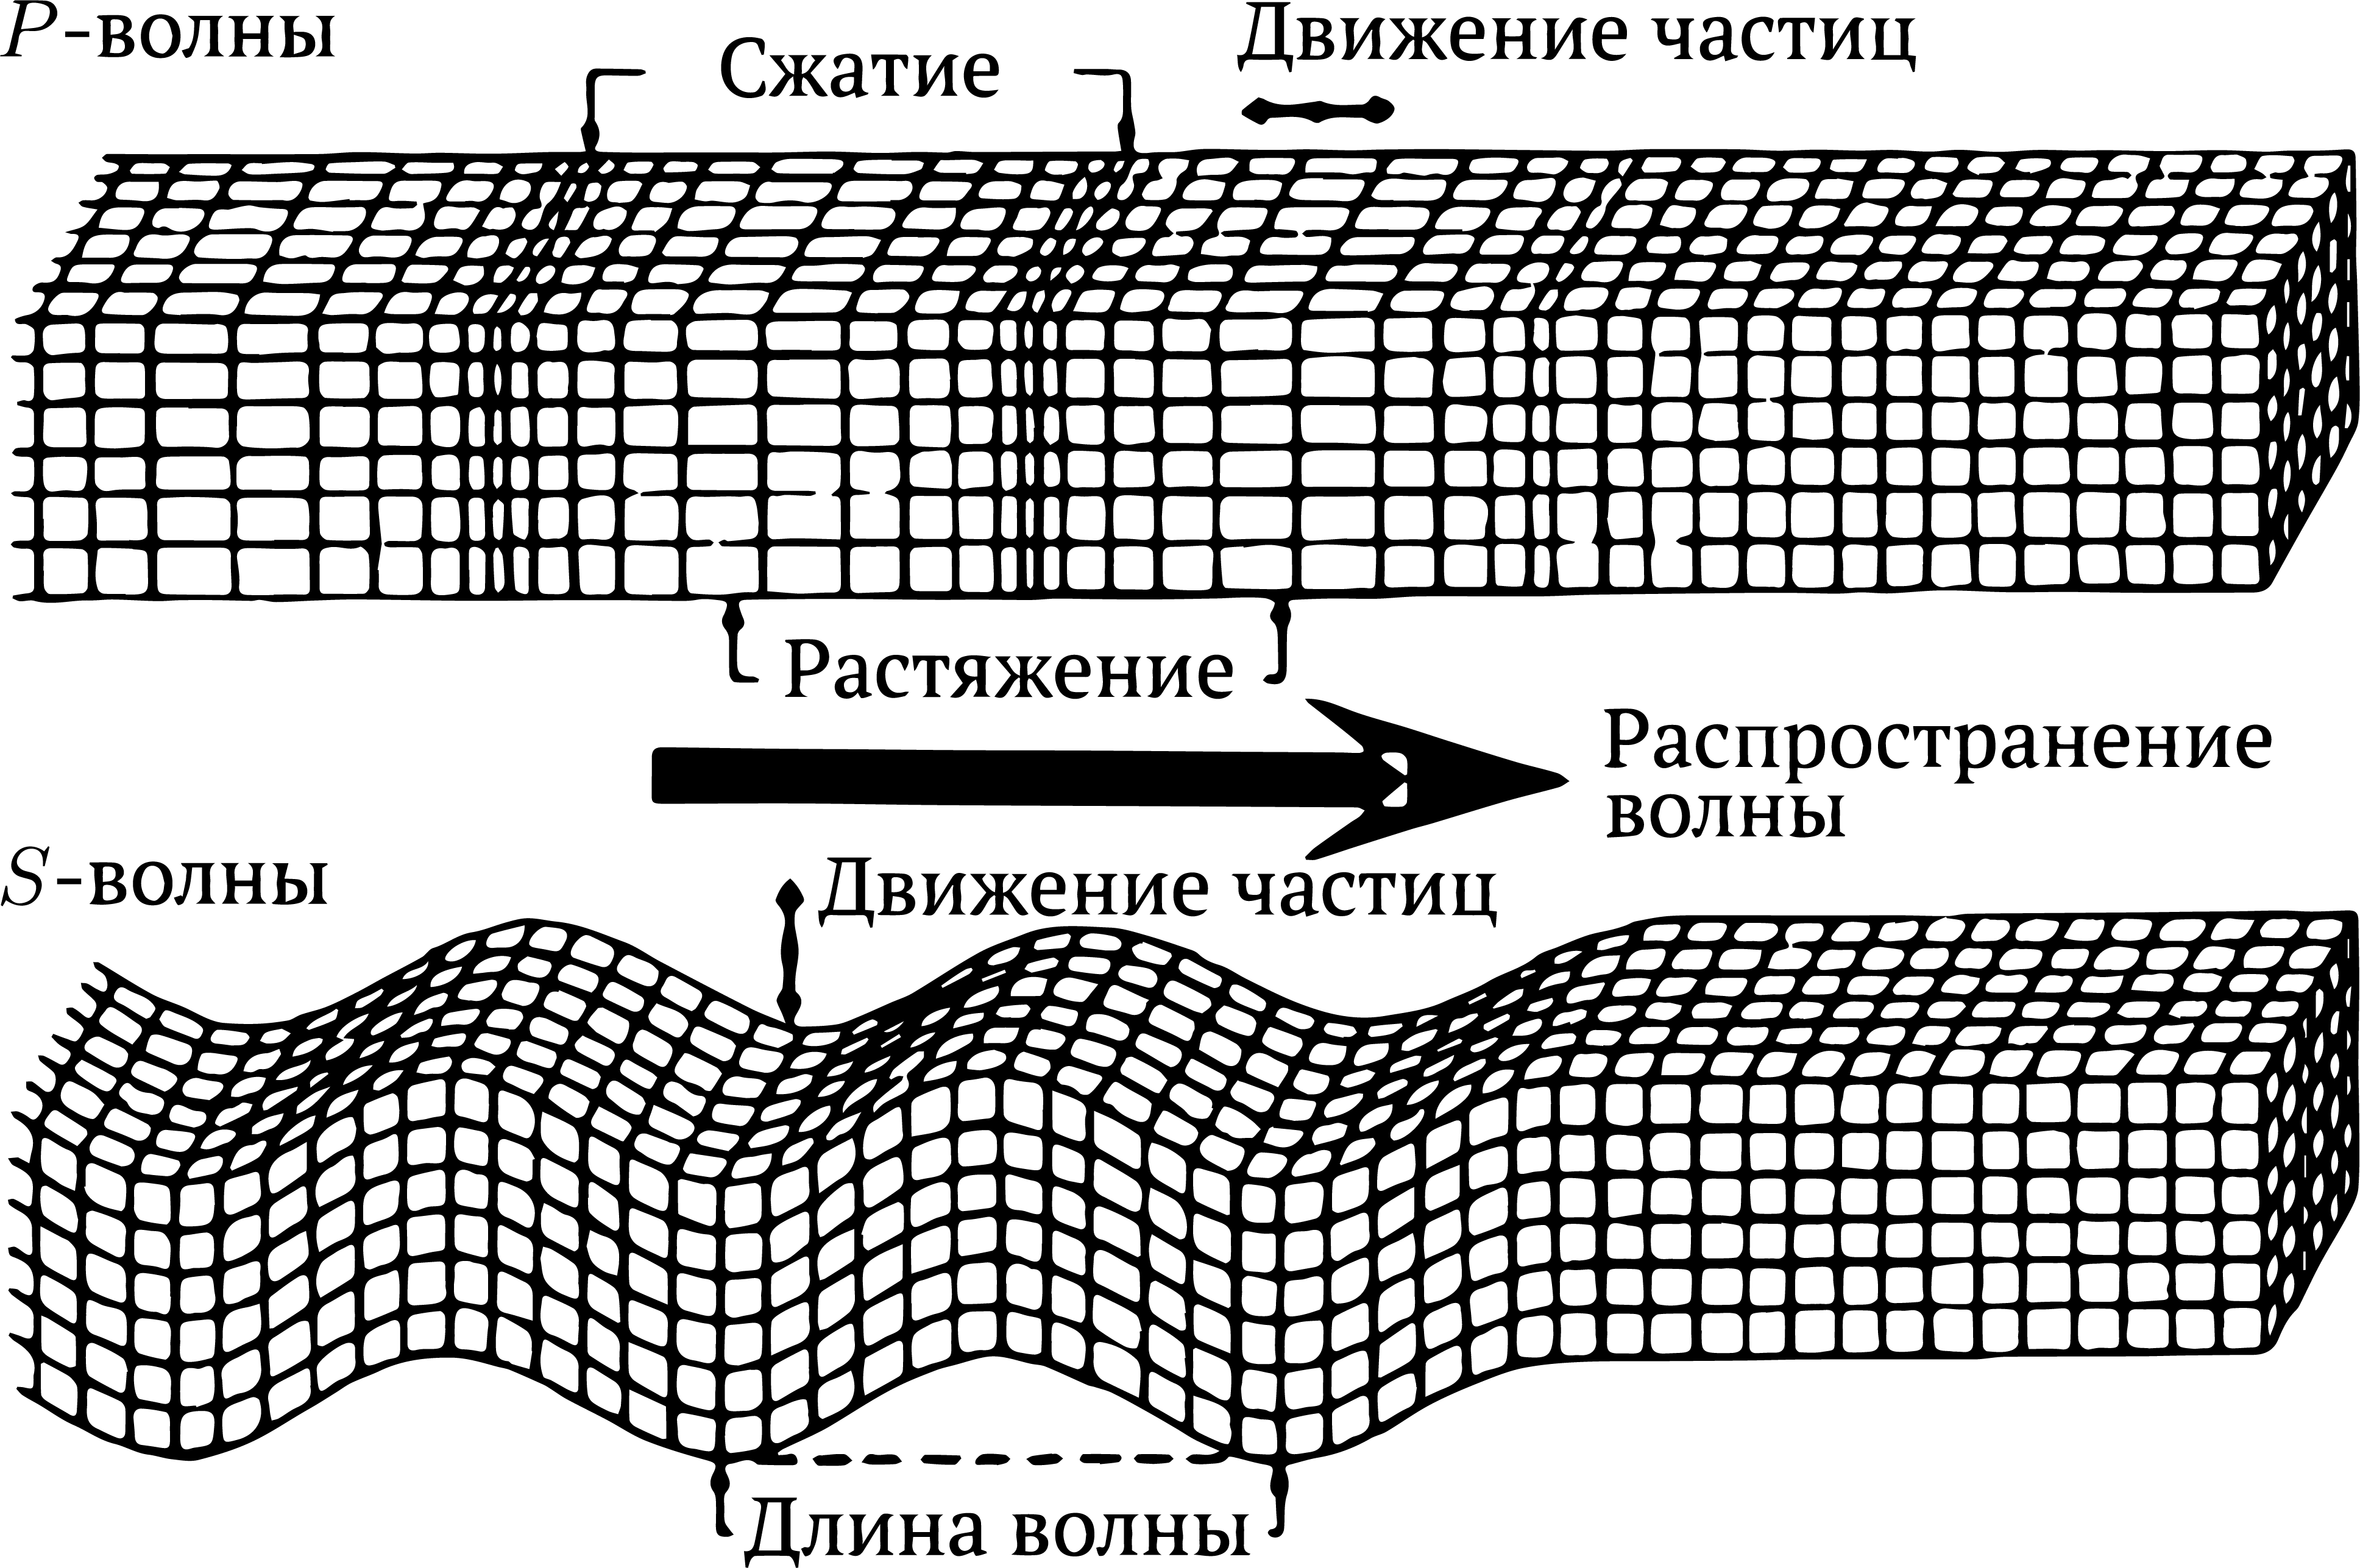
\includegraphics[width=\linewidth]{1-1}
		\caption{объемные волны}
		\label{1-1}
	\end{subfigure}
	\begin{subfigure}{.6\textwidth}
		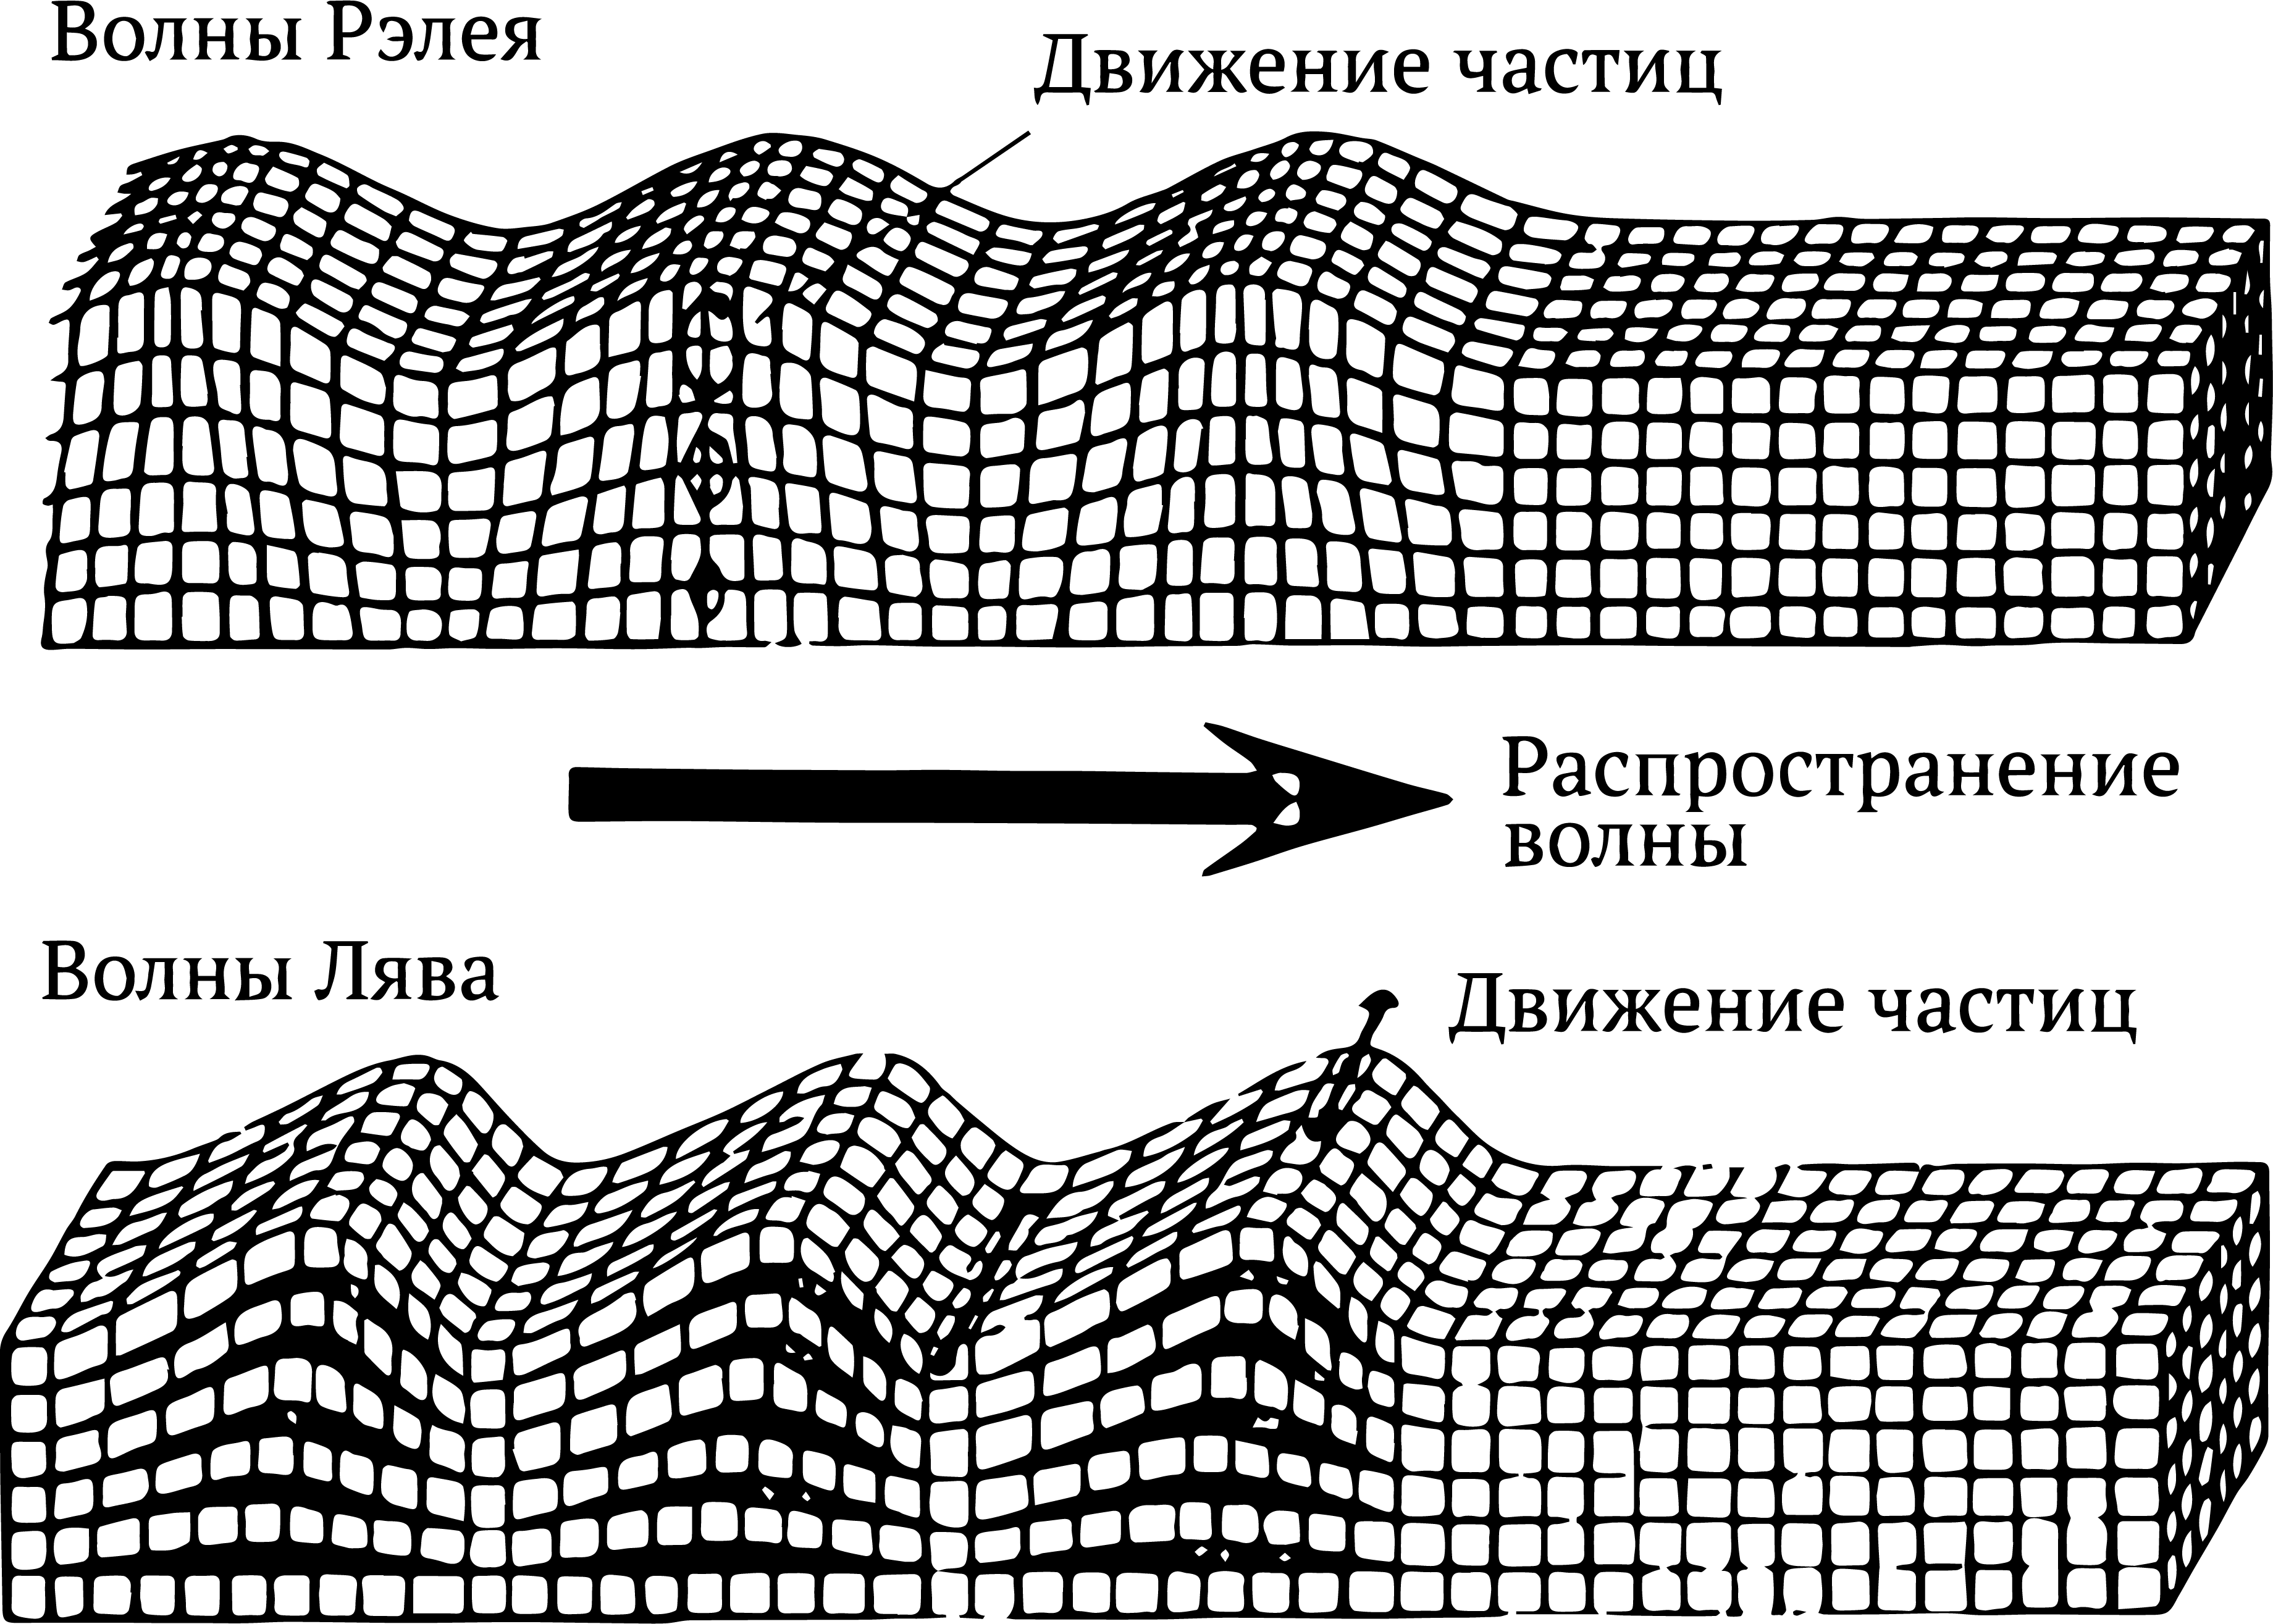
\includegraphics[width=\linewidth]{1-2}
		\caption{поверхностные волны}
		\label{1-2}
	\end{subfigure}
	\caption{Волны в упругой среде}
	\label{1}
\end{figure}



Законы распространения, преломления и отражения волн определяются лучевой или <<геометрической>> сейсмикой, аналогичной геометрической оптике. Основу этой теории образует принцип наименьшего времени Ферма (следствия принципа действия), согласно которому волна распространяется из одной точки в другую таким образом, чтобы время пробега было минимальным:
\begin{equation}
	\tau = \int\displaylimits_{1}^{2} \dfrac{ds}{c(\zeta)} \longrightarrow min.
\end{equation}

В сейсмологии удобно строить графики зависимости времени пробега объемных и поверхностных волн от эпицентрального расстояния. Эта зависимость называется годографом (Рис. \ref{2}).

\begin{figure}[H]
	\centering
	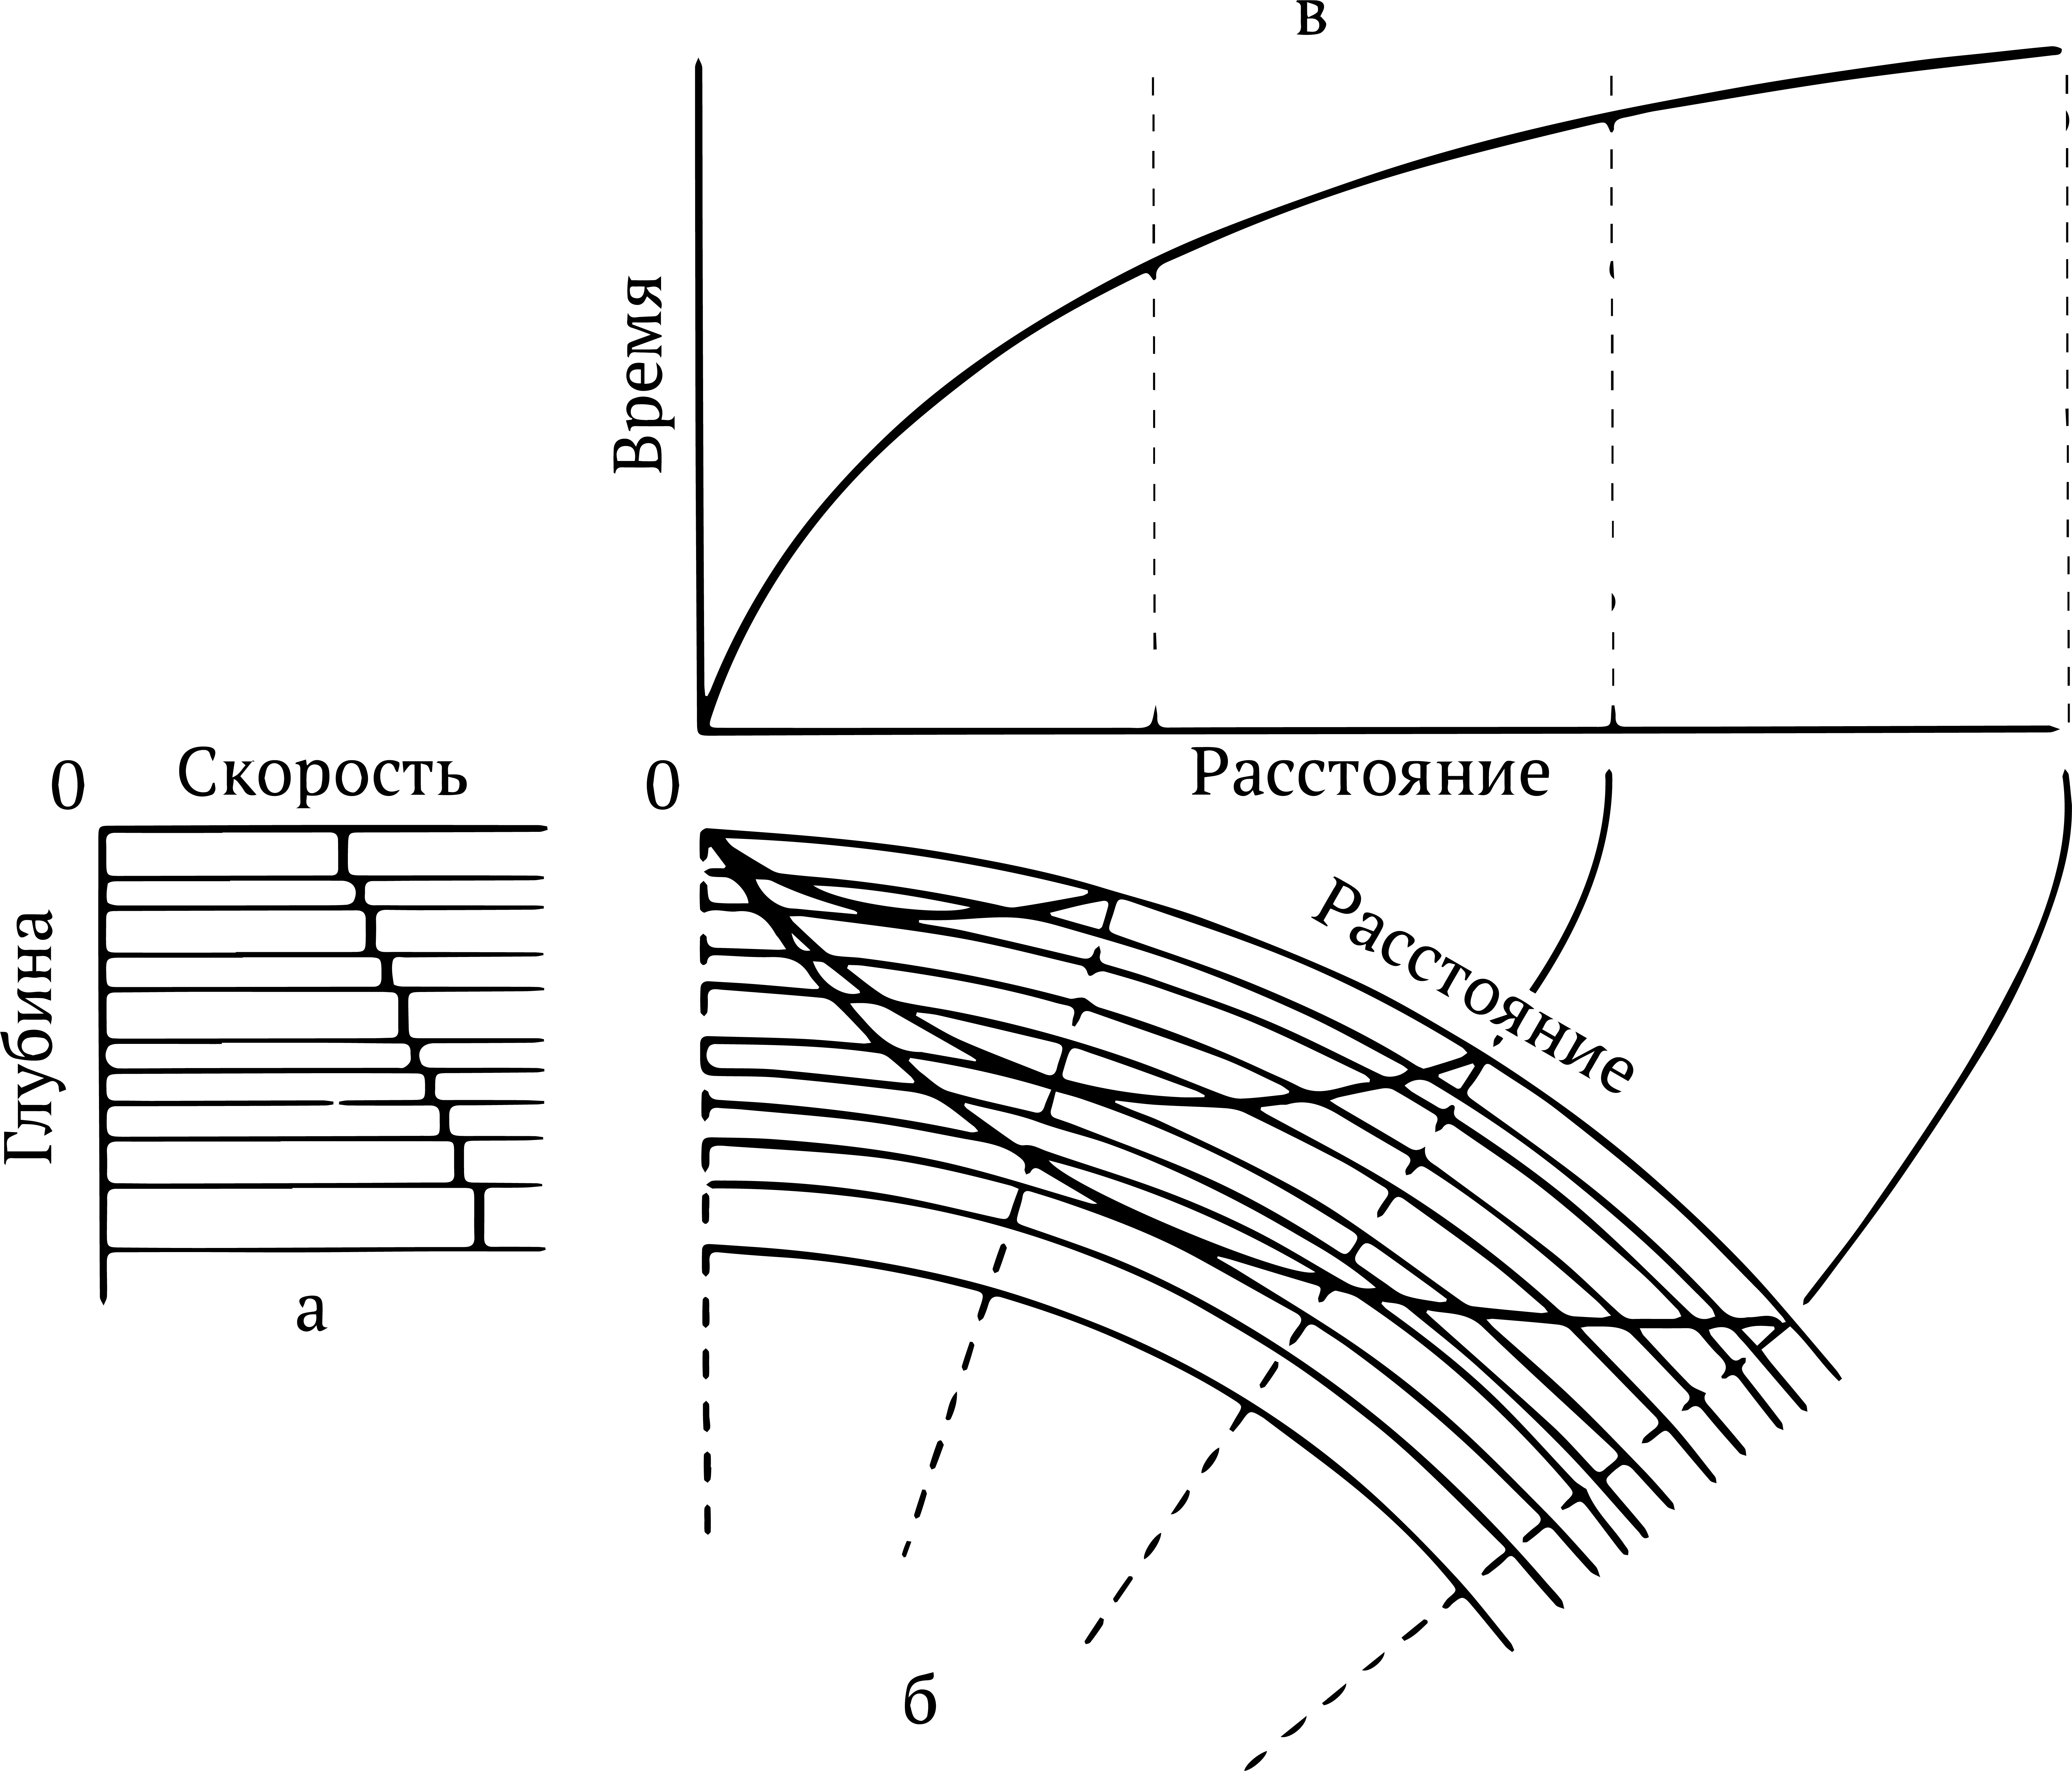
\includegraphics[width=.7\linewidth]{2}
	\caption{Принцип построения годографа:\\а - изменение скорости сейсмических волн с глубиной; б - ход лучей в сферической Земле; в - зависимость времени пробега волн от эпицентрального расстояние}
	\label{2}
\end{figure}

В сейсморазведке основным является метод отраженных волн (МОВ), меньшее применение имеет метод преломленных волн (МПВ). МОВ применяется в основном для изучения структур и расчленения разрезов осадочных толщ. Это основной метод поисков и разведки нефтегазоносных структур. МПВ чаще применяется при глубинных сейсмических исследованиях, определении глубины и рельефа кристаллического фундамента, изучении месторождений рудных ископаемых.

Обработка сейсмограмм и магнитограмм направлена на выделение нескольких полезных волн из сотен зарегистрированных. С помощью рациональной системы наблюдений и сложной цифровой обработки материалов подавить множество регулярных и нерегулярных волн-помех и выявить кинематические (время прихода) и динамические (амплитуда сигналов) характеристики волн. Затем их надо идентифицировать с однократными отраженными или преломленными волнами.

В результате обработки сейсмических данных получают времена $t$ прихода тех или иных волн на разных расстояниях от пунктов возбуждения $x$. По ним строятся (Рис. \ref{5}):
\begin{itemize}
	\item годографы волн (по горизонтали откладывается $x$, по вертикали вверх - $t$);
	\item профилограммы (по горизонтали - $x$, по вертикали вниз - записи всех полезных волн);
	\item временные разрезы (обычно МОВ и метод общей глубинной точки (МОГТ)): по горизонтали - $x$, по вертикали вниз - $t_0$, истинное или преобразованное.
\end{itemize}
Обработка заканчивается качественной интерпретацией выявленных однократных волн, т.е. дается характеристика изменения сейсмического разреза по горизонтали и вертикали. Особенно наглядны временные разрезы, на которых видны все структурные (геометрические) особенности разреза (Рис. \ref{3}).

\begin{figure}[H]
	\centering
	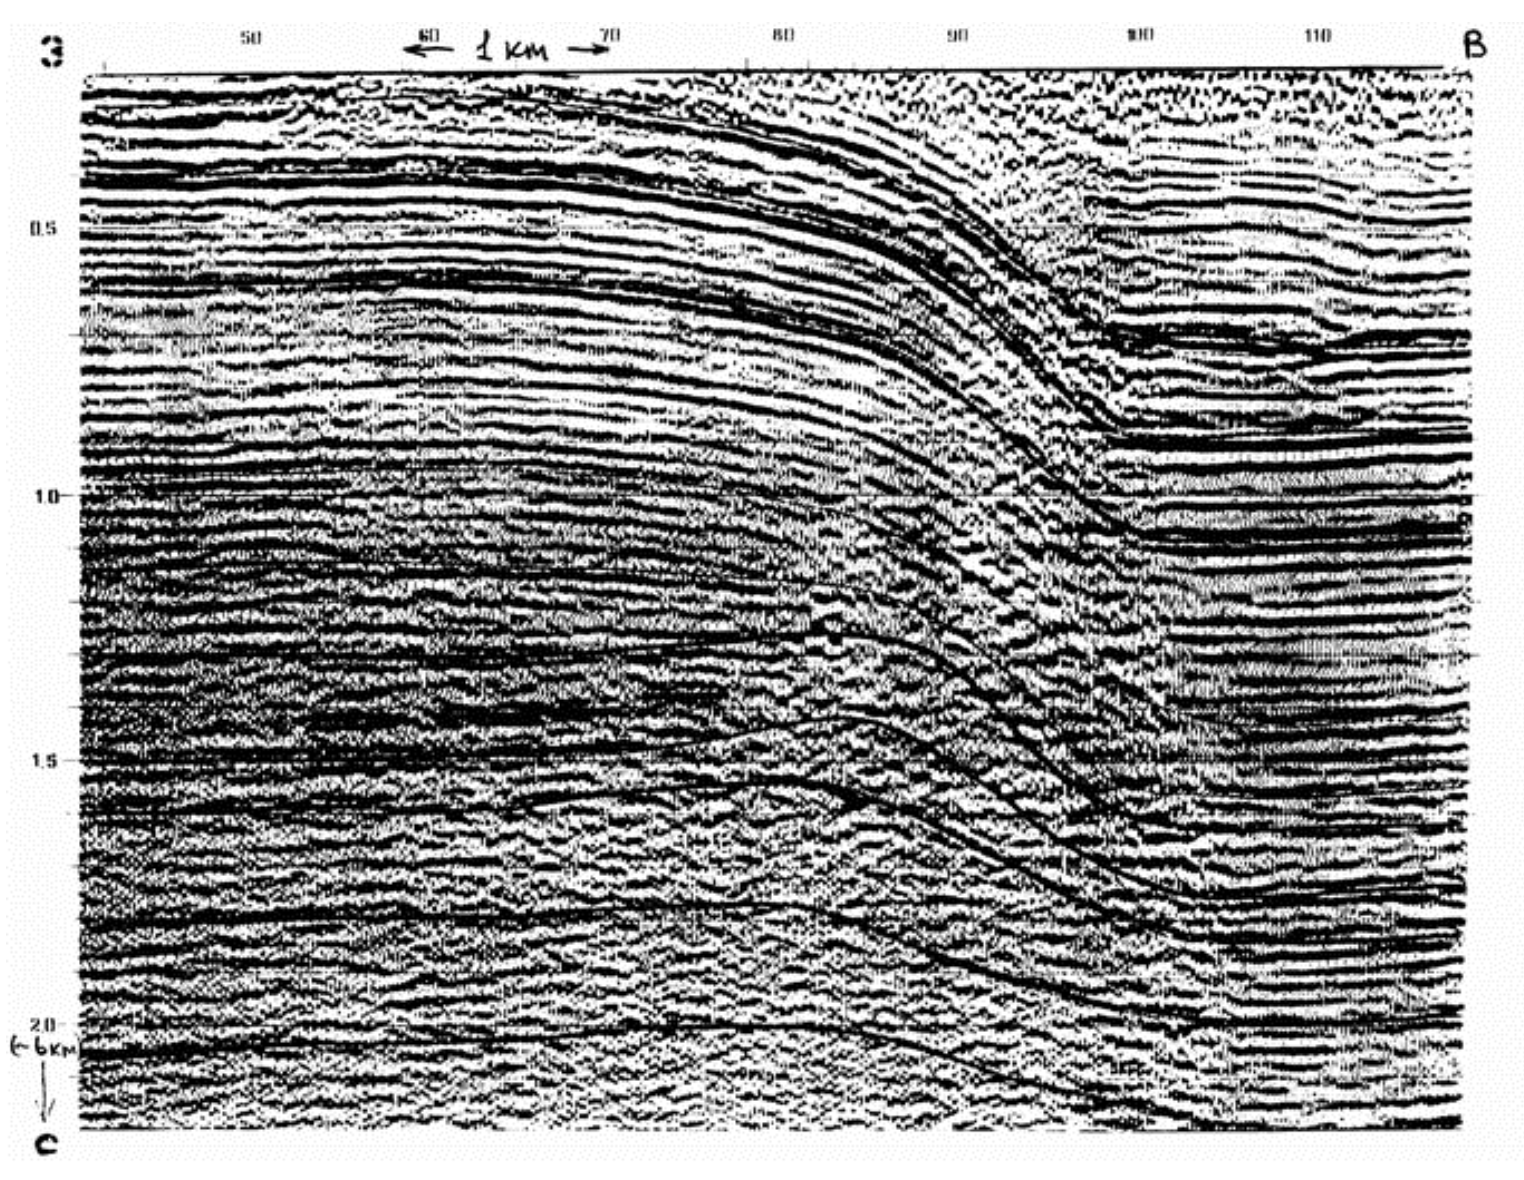
\includegraphics[width=.8\linewidth]{3}
	\caption{Временной разрез отраженных волн}
	\label{3}
\end{figure}



Можно вручную рассмотреть сейсмограммы, на которых непрерывная аналоговая запись представлена в видимой форме. В данном случае необходимо провести корреляцию, фазовую корреляцию, найти время прихода фазы той или иной волны к каждому сейсмоприемнику, определить статические поправки. Однако цифровая обработка сейсмических данных является более удобной. Ее основа - три математических операций: преобразование Фурье, свертка сигналов и корреляция. Целью разных методов цифровой обработки является увеличение отношения сигнал/помеха ($SNR$) для надежного отфильтрования кратных и других волн-помех, прокоррелирование оси синфазности полезных однократно отраженных или преломленных волн, определение времени их прихода по всем трассам и изменения амплитуд сигналов по ним.

\section*{Построение временных разрезов}
\addcontentsline{toc}{section}{Построение временных разрезов}

При обработке данных МОВ строятся временные разрезы (Рис. \ref{3}). Временной разрез - определенным образом преобразованные сейсмограммы, на котором записи отнесены к нулевому времени ($t_0$), т.е. времени пробега волны при нулевом удалении от приемника до источника. Для этого в наблюденные сейсмограммы вводятся кинематические поправки.

Такие разрезы автоматически получаются, когда сейсмоприемник располагается вблизи пункта возбуждения, а запись проводится одним сейсморегистрирующим каналом. При многоканальной автоматической записи строятся временные разрезы с помощью ЭВМ. Выделяя на временных разрезах оси синфазности, соответствующие временам прихода однократных отраженных волн, получаем линии $t_0$, каждая их которых соответствует одной из отражающих границ геологического разреза.

Временные разрезы, хотя и не несут информации о глубинах залегания отражающих границ, но дают представление об основных чертах геологического строения и являются важным результатом качественной интерпретации данных МОВ. Если средняя скорость не меняется вдоль профиля, то линия $t_0$ может быть непосредственно сопоставлена с отражающей границей. Зная среднюю скорость в толще нал отражающей границей и закон ее изменения со временем, легко перестроить временной разрез в глубинный.

\section*{Обработка данных метода общей глубинной точки}
\addcontentsline{toc}{section}{Обработка данных метода общей глубинной точки}

В методе общей глубинной точки (МОГТ) для каждой точки профиля ($x_i$) получается несколько ($N$) сейсмотрасс, т.е. запись с разных пунктов возбуждения (ПВ) и сейсмоприемников (СП), расположенных симметрично относительно $x_i$ (точки записи) (Рис. \ref{4}). При такой системе наблюдений во всех точках профиля последовательно могут располагаться ПВ и СП, а число таких перестановок равно кратности перекрытия ($N$).

\begin{figure}[H]
	\centering
	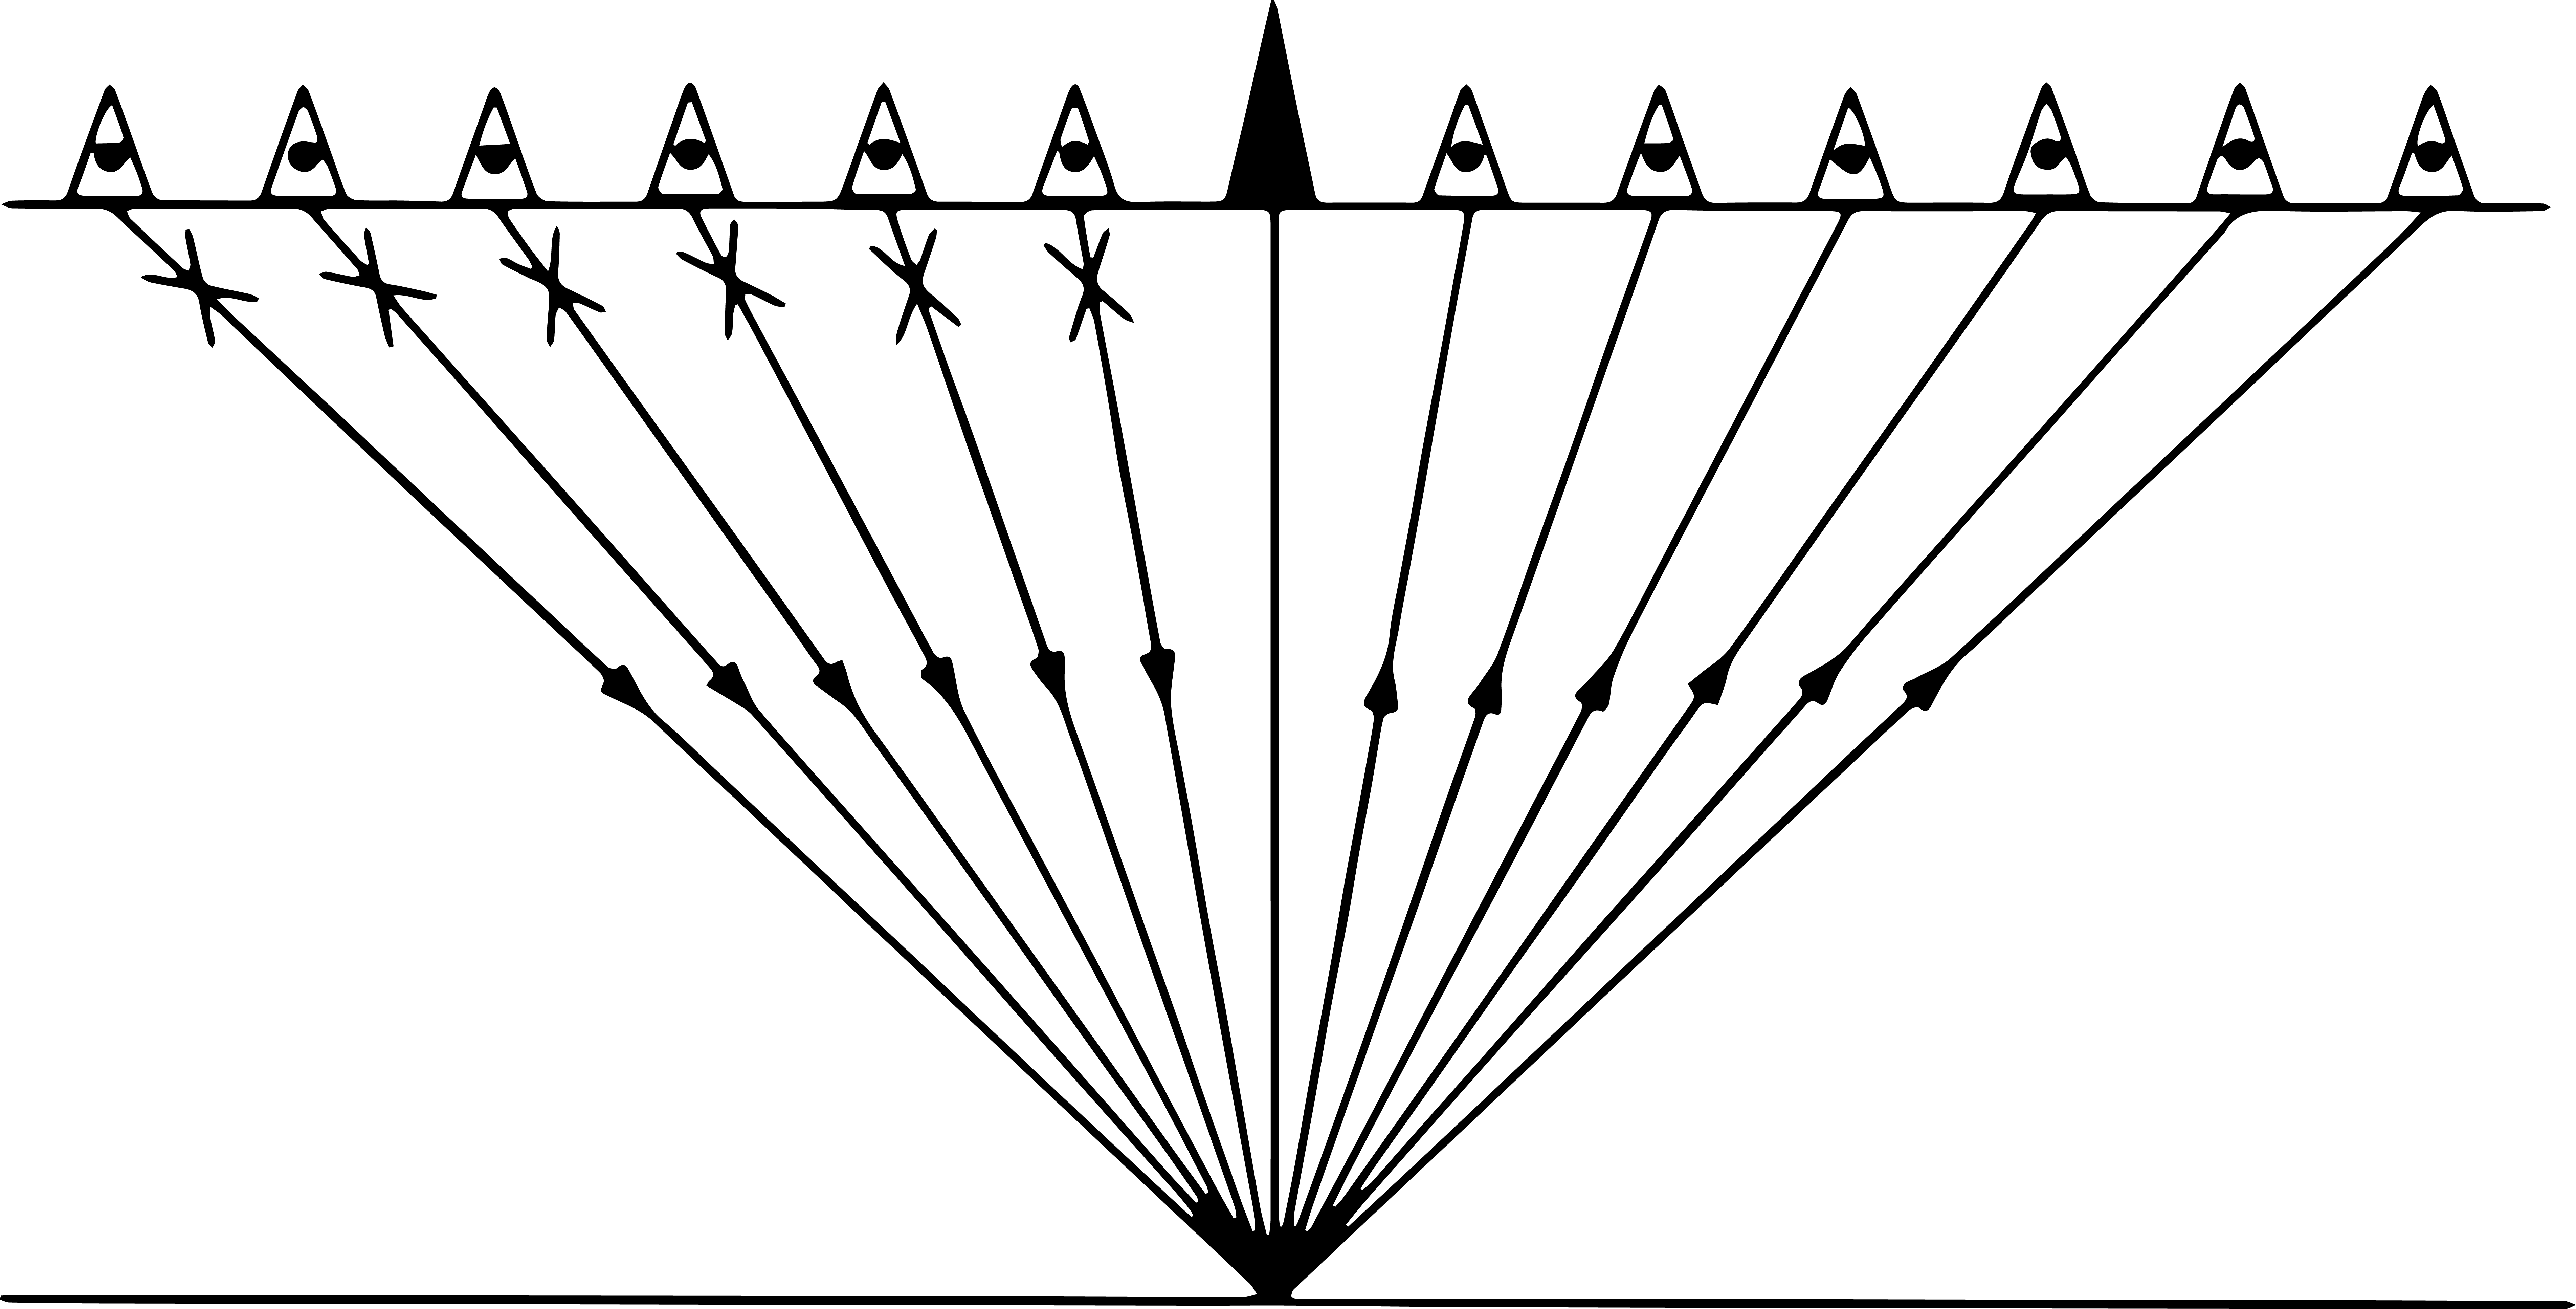
\includegraphics[width=.6\linewidth]{4}
	\caption{К обработке данных МОГТ}
	\label{4}
\end{figure}

Кроме однократных волн на сейсмограммах регистрируется множество многократно отраженных волн от различных границ раздела, поэтому они маскируют полезные однократные волны.

При обработке данных МОГТ осуществляется частисное подавление многократно отраженных волн. Для этого используются сложные многоступенчатые приемы суммирования всех $N$ сейсмотрасс с введением в них кинематическиз поправок и получением суммотрасс. Обработка требует больших расчетов и выполняется в автоматическом компьютерном режиме.

\section*{Количественная интерпретация данных сейсморазведки}
\addcontentsline{toc}{section}{Количественная интерпретация данных сейсморазведки}

Количественная интерпретация годографов и временных разрезов начинается с изучения скоростного разреза и определения средних скоростей ($v_{ср}$) толщ пород над каждой из выявленных отражающих и преломляющих границ. Далее временные разрезы преобразуются в глубинные, т.е. определяется геометрия разреза (глубины залегания, углы наклона ($\varphi$)) и распределение пластовых, средних, граничных скоростей по профилю в глубине.

Заключительным этапом является геологическое истолкование результатов, для чего используется вся геологическая информация, данные бурения и геофизических исследований в скважинах (ГИС). Оно заканчивается построением сейсмогеологических разрезов, называемых так потому, что это фактически структурно-геологические разрезы, но построенные по данным сейсморазведки и ГИС. Кроме того, строятся структурные карты.

Конечные результаты сейсморазведки всегда вероятностные, ибо обратная задача геофизики неоднозначна. Однако в сейсморазведке неоднозначность значительно меньше, а результаты точнее, чем в других геофизических методах. Качество построения структурных карт желательно проверять математическим моделированием, т.е. решением прямых задач для самых выраженных аномальных участков с построением синтетических сейсмограмм. Сравнение их с наблюдаемыми поможет оценить достоверность результатов.

Результаты изучения природы волн и идентификация сейсмических границ оказывается наиболее достоверными, если границы слоев, пластовых и интервальные скорости по данным полевых наблюдений увявзаны с данными вертикального сейсмического профилирования (ВСП), предназначенного для детального изучения сейесмических границ вблизи скважины, а также сейсмических и акустических исследований в самих скважинах. Совместный анализ сейсмических и геологических данных геофизиками и литологами позволяет проводить сейсмостратиграфическое изучение разреза. Суть его заключается в том, что на основе объективного материала о геометрии и скоростном строении неологического разреза получают сведения об условиях осадконакопления, сочленности и литологии контактирующих пород.

\begin{figure}[H]
	\centering
	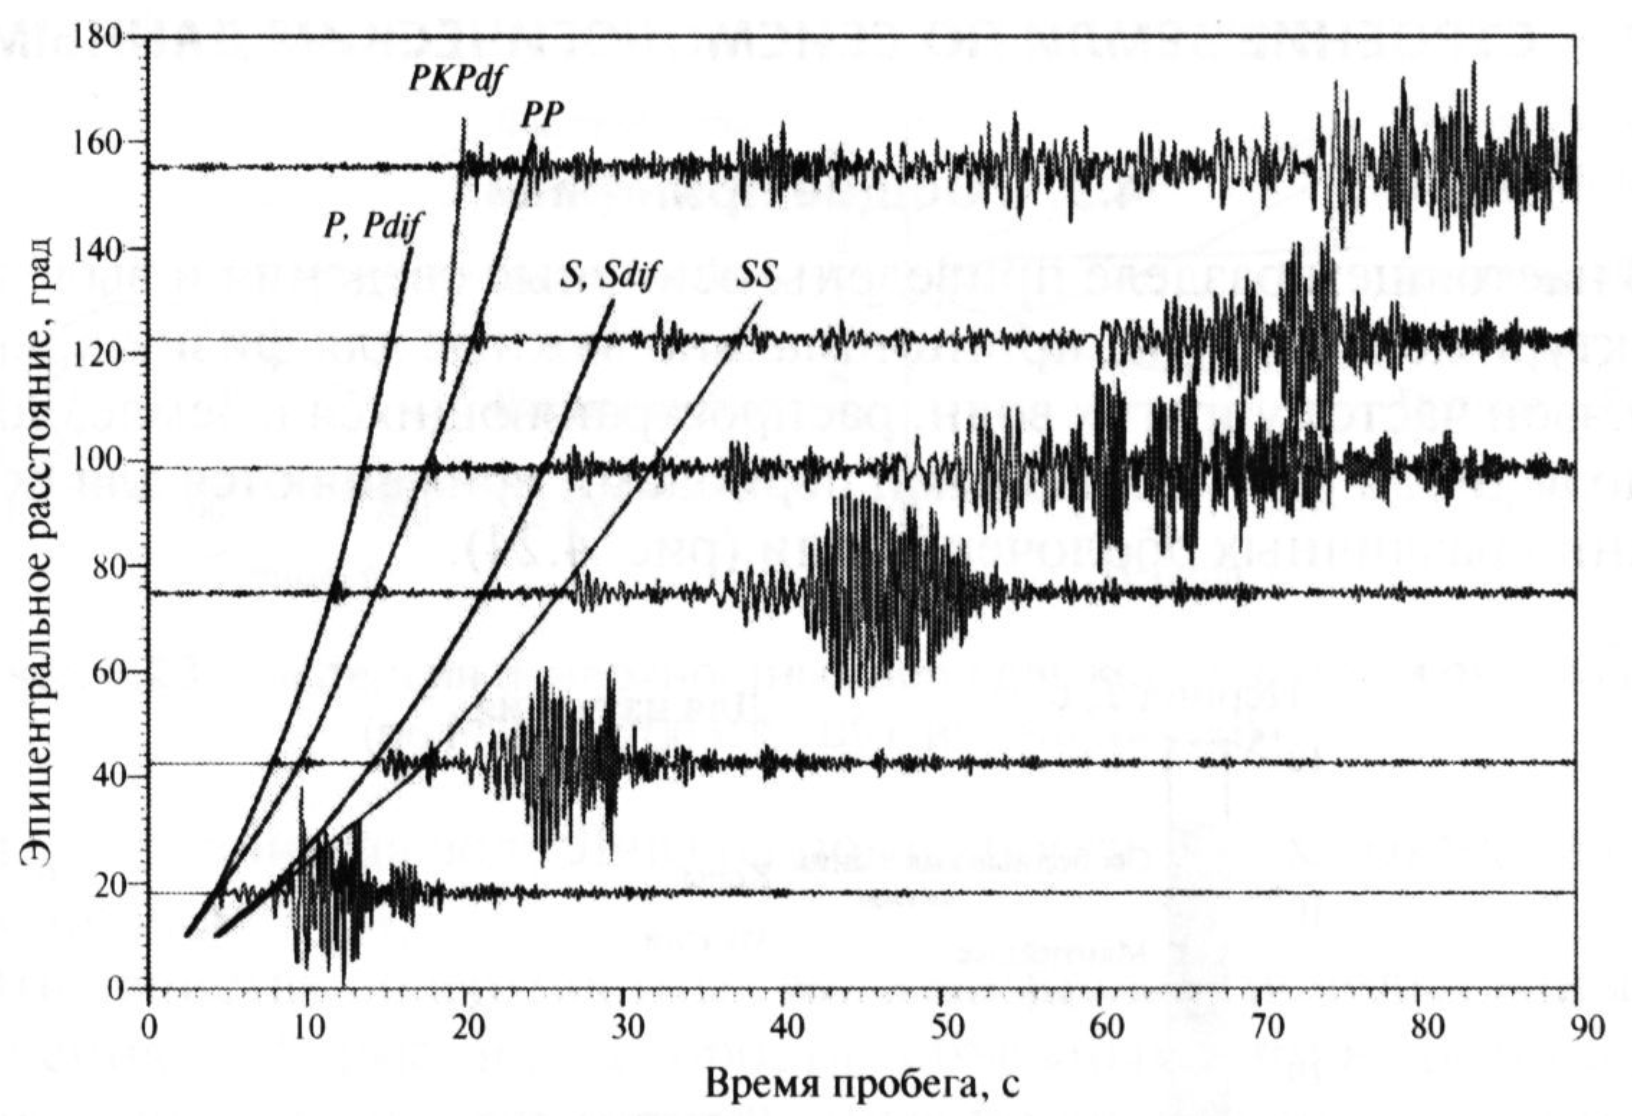
\includegraphics[width=.9\linewidth]{5}
	\caption{Построение годографа по записям землетрясений по станциям с эпицентральными расстояниями $18 - 157^{\circ}$:\\{\footnotesize показаны ветви, соответствующие разным сейсмическим фазам (по Bormann, 2012. Ch. 1, doi: 10.2312/GFZ.NMSOP-2\_ch1.P.11 с изменениями)}}
	\label{5}
\end{figure}